%auteur: Amaury JOLY
\subsubsection{Définition}
Les \gls{relay}s décentralisés sont des applications décentralisés permettant une intéropérabilités entre les \textit{\gls{blockchain}s} \cite{qin2018overview, westerkamp2022verilay,belchior2022survey}.
Leur but est de transmettre des informations entre des \textit{\gls{blockchain}s} distinctes (par exemple, \gls{Bitcoin} et \gls{Ethereum}). 
Les \gls{relay}s suivent une partie de l’état de leurs chaînes connectées afin de prouver l’existence de transactions d’une chaîne à l’autre.

\subsubsection{BTCRelay}
BTCRelay est un \textit{\gls{smart contract}} qui stocke les en-têtes de blocs \gls{Bitcoin} sur la \textit{\gls{blockchain}} \gls{Ethereum}. \cite{qin2018overview,belchior2022survey,btcrelay2022web,btcrelay2022git}
BTCRelay utilise ces en-têtes de blocs pour construire une mini-version de la \textit{\gls{blockchain}} \gls{Bitcoin}: une méthode utilisée par les 
portefeuilles légers \gls{Bitcoin} SPV. \footnote{\gls{Bitcoin} SPV signifie Simplified Payment Verification et c’est un moyen pour \gls{Bitcoin} de se 
développer et de se propager en fonctionnant sur des petits appareils, comme les téléphones portables et les ordinateurs portables.}
BTCRelay est open source, sans confiance et décentralisé. Il permet aux contrats \gls{Ethereum} de vérifier les transactions \gls{Bitcoin} sans aucun 
intermédiaire: en d’autres termes, les utilisateurs peuvent payer avec \gls{Bitcoin} pour utiliser les \gls{dApp}s \gls{Ethereum}. Il offre également la 
possibilité de relayer la transaction \gls{Bitcoin} à n’importe quel contrat \gls{Ethereum} et d’inspecter le dernier en-tête de bloc \gls{Bitcoin} stocké 
dans le contrat. Ce qui offre une possibilité d'opérabilité unidirectionnelle de \gls{Bitcoin} vers \gls{Ethereum}.\\

\begin{figure}[h!]
  \centering
  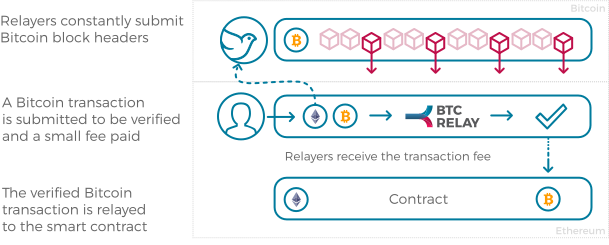
\includegraphics[scale=0.5]{decentralisation/btcRelay.png}
  \label{fig:btcRelay}
  \caption{BTCRelay}
\end{figure}

\begin{figure}[h!]
  \centering
  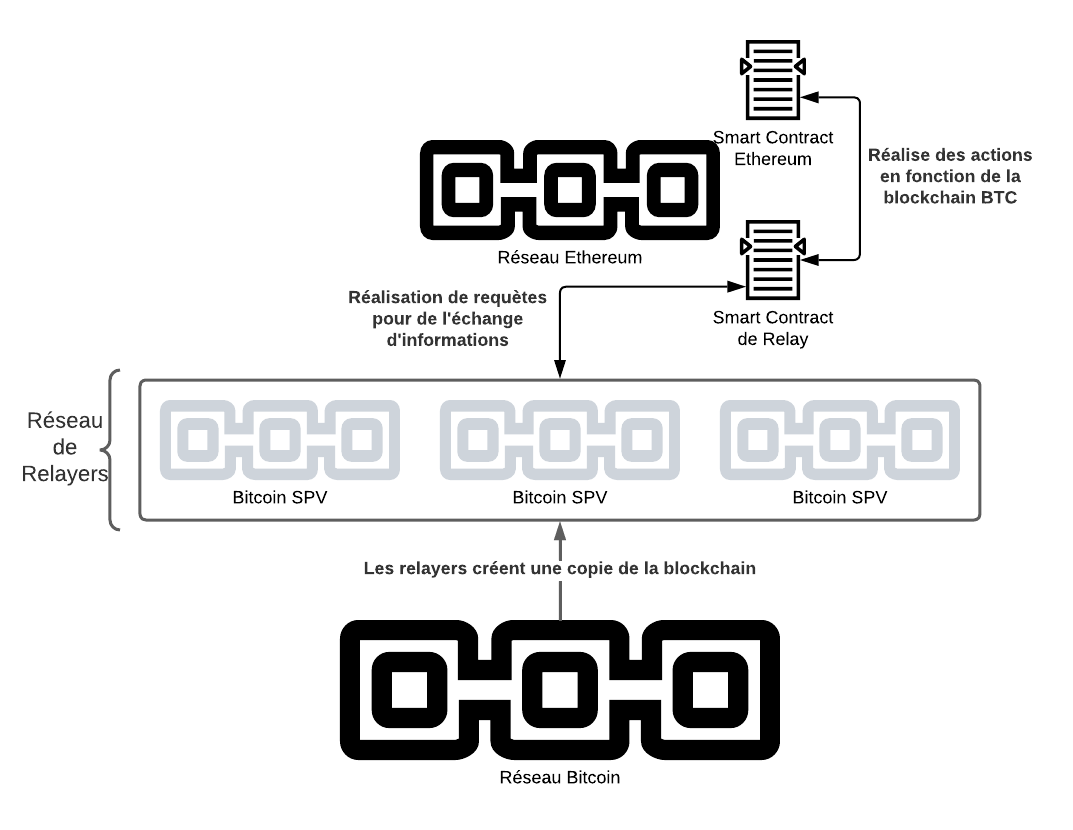
\includegraphics[scale=0.5]{decentralisation/btcRelay2.png}
  \label{fig:btcRelay2}
  \caption{BTCRelay}
\end{figure}

\pagebreak
\subsubsection{tBTC}
Un exemple d'usage de BTCrelay pour de l'echange \gls{cross-chain} est le projet tBTC, qui permet aux utilisateurs d’échanger des bitcoins contre des 
tokens ERC-20 représentant des bitcoins sur la \textit{\gls{blockchain}} Ethereum \cite{hildebrandt2020tokenization,lan2021horizon}. tBTC utilise un contrat intelligent 
appelé Deposit qui interagit avec un ensemble de signataires qui détiennent les bitcoins en garantie. 
Le contrat Deposit utilise BTCRelay pour vérifier les preuves SPV des transactions \gls{Bitcoin} et émettre ou 
brûler des \gls{actif} tBTC en conséquence. Ainsi, les utilisateurs peuvent profiter des avantages de la liquidité 
et de la programmabilité d’\gls{Ethereum} tout en conservant l’exposition au \gls{Bitcoin}. \\
Bien que tBTC se présente comme une solution décentralisée et sans confiance pour échanger des \gls{Bitcoin}s contre 
des tokens ERC-20, il existe certains défis et limites à son fonctionnement. 
Par exemple, tBTC repose sur un ensemble de signataires qui doivent déposer une garantie pour sécuriser les \gls{Bitcoin}s
verrouillés dans le contrat Deposit. Ceci expose les signataires à un risque financier permettant de limitter les risques de malveillance. 
De plus, tBTC nécessite que les signataires soient en ligne et disponibles pour répondre aux demandes de rachat des 
utilisateurs dans un délai donné. Si les signataires sont hors ligne ou malhonnêtes, les utilisateurs peuvent 
perdre l’accès à leurs \gls{Bitcoin}s ou être obligés d’attendre une longue période avant de pouvoir les récupérer. 
Les signataires sont choisis aléatoirement par un mécanisme appelé \textit{random beacon}, qui pondère la sélection en 
fonction du montant misé par les signataires potentiels. Cela vise à éviter la collusion ou la censure entre les 
signataires, mais cela n’exclut pas complètement la possibilité d’attaques sybil \footnote{Une attaque sybil est 
un type d’attaque sur un réseau pair à pair dans laquelle un attaquant crée un grand nombre d’identités fausses 
et les utilise pour gagner une influence disproportionnée sur le réseau} ou de corruption.

\begin{figure}[h!]
  \centering
  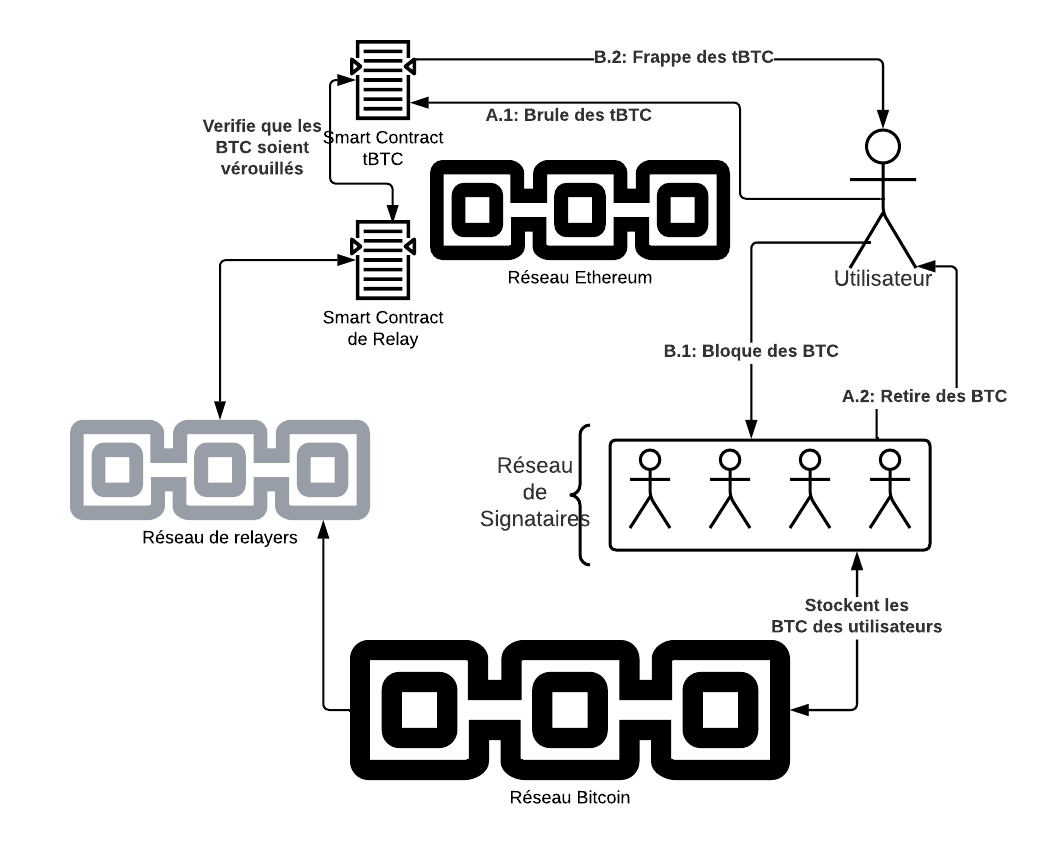
\includegraphics[scale=0.5]{decentralisation/tBTC.png}
  \label{fig:tBTC}
  \caption{tBTC}
\end{figure}
